
\paragraph{Conductivité thermique :}on la note $k$ ou $\lambda$ et elle s'exprime en W/K/m. Elle caractérise la capacité d'un matériau à conduire la chaleur (plus elle est élevée, plus le matériau conduit rapidement). Elle est assez liée à la conductivité électrique $\sigma$ du matériau (un matériau bon conducteur de chaleur est souvent également bon conducteur d'électricité), pour un \textbf{métal} la loi de Wiedmann-Franz affirme que :
%
\begin{equation}
    \frac{k}{\sigma~T} = L_0 = 2.44~10^{-8} W\Omega K^{-2}
\end{equation}
%
On parle aussi bien de problème de conduction que de diffusion, ici ces 2 termes sont identiques.


\paragraph{Loi de Fourier :}c'est la loi essentielle dans tout problème de diffusion (de la chaleur ou de la matière par exemple). Elle s'applique à tout matériau isotrope (une formulation plus complexe reste possible pour un matériau non isotrope). En thermique, elle représente la relation entre la densité de flux de chaleur $\vec{\phi}$ traversant un volume et le gradient de température au sein de ce volume :
%
\begin{equation}
    \vec{\phi} = - k \vec{\nabla}(T)
    \label{eq:fourier}
\end{equation}
%
La présence du signe négatif est physiquement logique : le flux va du chaud vers le froid alors que le gradient de température suit le sens inverse (il va des températures faibles aux températures élevées).
%
\begin{center}
    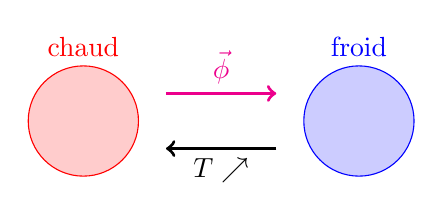
\begin{tikzpicture}[scale=0.7]
        \filldraw[fill=red!20,draw=red] (0,0) circle(1);
        \filldraw[fill=blue!20,draw=blue] (5,0) circle(1);
        \draw [red] (0,1) node[above] {chaud};
        \draw [blue] (5,1) node[above] {froid};
        % arrows
        \draw [magenta,->,very thick] (1.5,0.5) -- (3.5,0.5);
        \draw [->,very thick] (3.5,-0.5) -- (1.5,-0.5);
        % text
        \draw [magenta] (2.5,0.5) node[above] {$\vec{\phi}$};
        \draw (2.5,-0.5) node[below] {$T\nearrow$};
  \end{tikzpicture}
\end{center}


\paragraph{Diffusivité thermique :}c'est un rapport qu'on rencontre régulièrement en thermique, il caractérise également la capacité d'un matériau à diffuser la chaleur (présence importante de la conductivité) :
%
\begin{equation}
    \alpha = \frac{k}{\rho c_p}
\end{equation}


\paragraph{Équation de la température :}
%
\begin{equation}
    \rho~c_p \frac{DT}{Dt}
    = \vec{\nabla} \cdot \vec{\phi} %k \nabla^2 T
    + \rho~q_*
    + \vec{\vec{\tau}} : \vec{\vec{D}}
    + \beta T\frac{Dp}{Dt}
\end{equation}
%
On note que d'après \eqref{eq:fourier} on a : $\vec{\nabla} \cdot \vec{\phi} = - k \nabla^2 T$.

La géométrie du problème et les hypothèses physiques nous mènent souvent à adopter une forme simplifiée de cette équation. Dans un cas sans mouvement de fluide (conduction pure) et sans apport de chaleur, on a :
%
\begin{equation}
    \frac{\partial T}{\partial t}
    = \alpha \nabla^2 T
\end{equation}

Un élément utile à retenir : la diffusion de chaleur tend à lisser le champ de température, à diminuer les écarts de température. Les pics de chaleur initiaux sont étalés en distance avec le temps, et cette distance à l'instant $t$ est de l'ordre de $\sqrt{\alpha~t}$ (en m).


\paragraph{Nombre de Péclet :}il représente le rapport entre effets d'inertie et effets thermiques, c'est le pendant du nombre de Reynolds dans le domaine de la thermique
%
\begin{equation}
    Pe = \frac{Ul}{\alpha}
\end{equation}
%
On observe aussi l'existence de couches et sillages thermiques autour des obstacles à $Pe$ élevé (attention ces couches sont à distinguer des couches limites visqueuses).

\paragraph{Nombre de Prandt :}il est définit comme le rapport des diffusivités visqueuse et thermique, il représente ainsi l'importance relative entre effets visqueux et thermiques.
%
\begin{equation}
    Pr = \frac{\nu}{\alpha}
       = \frac{\mu~c_p}{k}
       = \frac{Pe}{Re}
\end{equation}
%
Il est très élevé ($10^3$) dans le cas d'une huile (grande viscosité) et très faible ($10^{-2}$) pour un métal liquide (excellents conducteurs thermiques et peu visqueux). Pour un gaz, il est d'environ $0.7$, et pour l'eau il est compris entre $1$ et $10$.

%\begin{center}
%  \begin{tikzpicture}
%  \fill[fill=gray!20] (-4,2) -- (0,2) -- (0,-1) -- (-4,-1);
%  \fill[fill=gray!40] (0,2) -- (4,2) -- (4,-1) -- (0,-1);
%  \draw [very thick,->] (-4,0) -- (4,0);
%  \draw (0,-1) -- (0,2);
%  \draw (0.5,0) node[below] {$x=0$};
%  \draw (-2,1) node[above] {$T_A(x)$};
%  \draw (2,1) node[above] {$T_B(x)$};
%  \end{tikzpicture}
%\end{center}


% ------------------------------------------------------
\subsection{Flux de conduction et convection}
La convection est le second grand phénomène de la thermique, après la conduction. Elle se définit comme un transfert d'énergie directement lié à un transport de masse. Ainsi, dès qu'il y a mouvement, il y a convection, le cas le plus courant est celui d'un fluide en mouvement par rapport à un solide (on sera dans ce cadre ici). On distingue 2 types de convection : la forcée et la libre (ou naturelle), décrites ci-dessous. Le coefficient de convection $h$ est dans tous les cas un nombre important dans la prédiction des comportements convectifs.

Ce nombre $h$ intervient dans l'écriture des flux de chaleur aux parois. Ces flux aux parois peuvent définir les conditions limites des problèmes thermiques. Pour une paroi plane située à l'abscisse $x_0$ et séparant les milieux 1 et 2, les densité de flux s'écrivent ainsi :
%
\begin{align}[left=\empheqlbrace]
    &\phi_{\text{conduction}}
    = - k_1 \left. \frac{\partial{T_1}}{\partial{x}} \right|_{x=x_0}
    = - k_2 \left. \frac{\partial{T_2}}{\partial{x}} \right|_{x=x_0} \\
    &\phi_{\text{convection}}
    = h_{12} \left( T_2 - T_1 \right)_{x=x_0}
    \label{eq:fluxth}
\end{align}


% ------------------------------------------------------
\subsection{Convection forcée :}
Le phénomène de convection forcée apparaît lorsque le fluide est mis en mouvement par
l'écoulement du fluide est , par une pompe par exemple. Ce mouvement forcé du fluide et à l'origine d'échange convectifs avec le solide en contact. Cependant, au sein même du fluide, son mouvement fait déjà apparaître un terme advectif dans son équation de la chaleur. Ce terme est dû à la dépendance de $T$ en temps, et témoigne du transport de la chaleur avec l'écoulement à la vitesse $\vec{U}$ :
%
\begin{equation}
    \rho~c_{p} \left( \frac{\partial T}{\partial t}
    + \vec{U} \cdot \vec{\nabla} T \right)
    = - \vec{\nabla} \cdot \vec{\phi}
\end{equation}

\paragraph{Nombre de Nusselt :}il est défini comme le rapport entre le gradient de température à la paroi et le gradient de température "élargi". Il permet de calculer le coefficient de convection $h$.
%
\begin{equation}
    Nu = \frac{h~l}{k_f}
       = \frac{\left. \frac{\partial{T}}{\partial{x}} \right|_{x=x_0}}
              {\left( T_f - T_s \right)/l}
\end{equation}
%
avec $k_f$ la conductivité du fluide en mouvement. Une analyse dimensionnelle (basée sur le théorème de Vaschy-Buckingham et détaillée en \cite{battaglia2010introduction}) affirme que ce nombre peut être écrit en fonction des nombres de Reynolds $Re$ et Prandt $Pr$ (ou indifféremment Péclet $Pe$).

On retrouve l'écriture de $\phi_{\text{convection}}$ \eqref{eq:fluxth} ainsi :
%
\begin{equation}
    \phi = - k_f \left. \frac{\partial{T}}{\partial{x}} \right|_{x=x_0}
         = k_f \frac{Nu}{l} \left( T_s - T_f \right)
         = ...
\end{equation}

En conclusion, pour un volume $V$ de fluide en mouvement et en contact avec un solide sur une surface $S$, l'équation de la chaleur a la forme suivante :
%
\begin{equation}
    \rho~c_p \left( \frac{\partial T}{\partial t}
    + \vec{U} \cdot \vec{\nabla} T \right)
    = \frac{h S}{V} \left( T_s - T \right)
\end{equation}
%
$S$ est bien la surface de contact entre fluide et solide. Il existe de nombreuses prescriptions empiriques du nombre de Nusselt $Nu$ pour des convections forcées internes (fluide dans une conduite) ou externes (solide plongé dans un écoulement).


% ------------------------------------------------------
\subsection{Convection libre :}
Ici le fluide est initialement au repos, et c'est le transfert de chaleur qui le met en mouvement. Un gradient de température apparaît au sein du fluide, et la dépendance de sa densité $\rho$ avec la température est à l'origine d'un mouvement du fluide, par poussée d'Archimède (le fluide plus léger monte etc). Ce mouvement du fluide est dissipé par effets visqueux et par diffusion thermique (la diffusion tend à uniformiser la température, donc à réduire les différences de densité).

On peut également définir un nombre de Nusselt $Nu$, mais il ne sera plus exprimé en fonction de $Re$, car la vitesse $\vec{U}$ n'a pas de sens en convection libre (elle n'est pas nulle, mais il est impossible de vraiment la déterminer). Le nouveau coefficient important en convection libre est le coefficient de dilatation thermique $\beta$ du fluide (en K\up{-1}) :
%
\begin{equation}
    \beta = \frac{1}{V} \left( \frac{\partial V}{\partial T} \right)_p
          = - \frac{1}{\rho} \left( \frac{\partial \rho}{\partial T} \right)_p
\end{equation}
%
Ce coefficient vaut $\beta = 1/T$ pour un gaz parfait. Dans le cadre de notre étude, on suppose que les variations de densité $\rho$ avec la température $T$ sont faibles et linéaires en $T$ :
%
\begin{align}
    &\rho(T) = \rho_0(T_0) \left( 1 - \beta(T-T_0) \right) \\
    \notag &\beta (T-T_0) \ll 1
\end{align}

\paragraph{Nombre de Grashof :}il compare les forces visqueuses aux forces de gravité
%
\begin{equation}
    Gr = \frac{1}{\nu^2}\beta g l^3 \Delta T
\end{equation}
%
On peut exprimer $Nu$ en fonction de $Gr$ et $Pr$, ces relations sont déterminées expérimentalement et sont différentes selon la géométrie du problème.

\paragraph{Nombre de Rayleigh :}il est très lié à $Gr$ et permet de déterminer le régime d'écoulement en convection libre, on peut aussi déterminer $Nu = f(Pr,Ra)$
%
\begin{equation}
    Ra = Pr.Gr
       = \frac{1}{\nu\alpha}\beta g l^3 \Delta T
\end{equation}

Les prescriptions donnant le nombre de Nusselt $Nu$ sont encore plus rares et empiriques que dans le cas de la convection forcée. On remarque que la convection libre externe est plus aisée à étudier que la convection libre interne (où la fermeture du fluide implique beaucoup d'effets difficilement prévisibles). Également, le caractère chaud ou froid d'une source a son importance : comme le fluide monte généralement avec la chaleur, l'inversion des sources crée un tout nouveau problème.


% ------------------------------------------------------
\subsection{Convection mixte :}

En convection forcée et régime laminaire, il peut se créer dans certaines conditions un mouvement des particules dû à la convection naturelle (ce mouvement s'ajoute au mouvement forcé des particules). Si le nombre de Prandtl $Pr$ est très faible ($10^{-2}$ ou moins), cela signifie que la couche thermique est plus épaisse que la couche visqueuse. Un gradient de température apparaît dans tout l'écoulement, et le mouvement des praticules est influencé par les variations de densité et les forces d'Archimède.

Il existe un autre critère simple pour déterminer l'importance relative de la convection forcée et de la convection libre sur une étude : le nombre adimensionné de Richardson $Ri$.
%
\begin{equation}
    Ri = \frac{Gr}{Re^2}
\end{equation}
%
La convection est principalement forcée pour $Ri \ll 1$ (on peut négliger la convection naturelle). Pour $Ri \gg 1$, la convection naturelle prend le dessus, le moteur mécanique de la convection forcée n'a plus d'influence sur l'écoulement. Entre ces 2 cas, pour $Ri \simeq 1$, les 2 phénomènes participent aux échanges de chaleurs, et on ne peut pas se permettre de négliger l'un des deux. La convection naturelle peut alors améliorer les échanges de chaleur ou s'y opposer, cela dépend notamment du sens de l'écoulement relativement à la gravité. On peut définir un nouveau nombre de Nusselt qui témoigne de l'influence des 2 phénomènes :
%
\begin{equation}
    Nu_{\text{total}} = \left( Nu_{\text{forcée}}^n \pm Nu_{\text{naturelle}}^n \right)^{1/n}
\end{equation}
%
Le signe devant $Nu_{\text{naturelle}}$ témoignent de l'influence positive ou négative de la convection naturelle. $n$ vaut 3 pour un mouvement vertical et 4 pour un mouvement horizontal.

